\subsection{Which sentences of the report survive}

\begin{table}[htbp]
\centering\small
\begin{tabular}{llcc}
\toprule
& claim (as written in the report, more or less) & true on & 95\% interval \\
\midrule
R1 & robot TD: $\eta = 0.01$ gives the smallest error for s/w & 100 & [0.96, 1.00] \\
R2$^\dagger$ & robot TD: $\eta = 0.01$ gives the smallest error for s/s & 63 & [0.53, 0.72] \\
R3 & robot TD: $\eta = 0.01$ gives the smallest error for s/re & 100 & [0.96, 1.00] \\
R4 & robot TD: with $1/n$ the error for s/re is still above 1 & 100 & [0.96, 1.00] \\
R5 & robot TD: s/s is the hardest policy for every constant step & 100 & [0.96, 1.00] \\
R6 & robot MC: all six true values are inside the 95\% intervals & 80 & [0.71, 0.87] \\
R7 & robot MC $\varepsilon$-greedy with the real return finds s/re & 100 & [0.96, 1.00] \\
R8 & robot MC $\varepsilon$-greedy with the immediate reward finds s/w & 100 & [0.96, 1.00] \\
S1 & student TD: $\alpha = 0.01$ gives the smallest error & 88 & [0.80, 0.93] \\
S2 & student TD: $1/n$ is worse than $0.01$ & 88 & [0.80, 0.93] \\
S3 & student Q-learning: the three $\alpha$ all end on W/W/W/R & 88 & [0.80, 0.93] \\
S4 & student Q-learning: $\alpha = 0.5$ ends on W/W/W/R & 89 & [0.81, 0.94] \\
S5 & student Q-learning: $\alpha = 0.01$ is stable after 2\,500 to 4\,500 episodes & 97 & [0.92, 0.99] \\
S6 & student Q-learning: $Q(2, R)$ is at least 3 below $q^*$ with $\alpha = 0.01$ & 7 & [0.03, 0.14] \\
\bottomrule
\end{tabular}
\caption{Number of seeds (out of 100) on which each claim of the report holds, with Wilson intervals for the frequency. $^\dagger$R2 is not in the report itself, we wrote it in the French follow-up from a mean over 30 seeds.}
\label{tab:claims}
\end{table}

Table~\ref{tab:claims} sorts itself quite naturally in three groups. Seven claims hold on (almost) every seed: R1, R3, R4, R5, R7, R8 and S5. These are the ones where the effect is large, for example $\eta = 0.01$ against the other steps for s/w and s/re, or the policy found by Monte Carlo control. Five claims are true most of the time but not always (between 80 and 89 seeds). And two are really fragile.

The first fragile one is R2. For the policy s/s, which has the noisy breakdowns, $\eta = 0.01$ is the best step on only 63 seeds, and on the 37 others it is the step $1/n$. We did not write this sentence in the report, we wrote it in the French follow-up because it is true on average over 30 seeds (here $0.55$ against $0.80$ over 100 seeds). Funny enough, the seed of the report is one of the 37 where $1/n$ wins ($0.39$ against $0.46$), so the table of the report already contradicted it and we did not notice. On average the claim is right, seed by seed it is not far from a coin flip, and the probability that one random run of $\eta = 0.01$ beats one random run of $1/n$ is only $0.63$.

The second one is S6. In the report we found $Q(2, R) = 10.3$ against $q^* = 15.29$ and explained it by the fact that this action is rarely tried. The explanation is fine, but over 100 seeds the mean is $14.5 \pm 1.5$ and only 7 seeds are 3 or more below $q^*$. Our seed 32 is part of the 100 (we used seeds 1 to 100) and it gives the lowest value of all of them. So the size of the effect we commented on was the worst case.

Two of the ``mostly true'' claims are worth a word because the reason is not just noise. For R6 (all true values inside the Monte Carlo intervals) we read the intervals at two decimals like in the report; strictly it is 0 out of 100 because of the truncation bias explained in the French follow-up. And 80 out of 100 is about what one should expect anyway: five of the six intervals are real 95\% intervals (in our runs each one covers the true value between 92\% and 99\% of the time), and $0.95^5 \approx 0.77$. Looking at six intervals and finding them all fine is not a 95\% event, it is a small multiple-testing problem that we did not think of when writing.

For S3 and S4 the explanation is even simpler. With $\alpha = 0.5$ the share of the last 5\,000 episodes where the greedy policy is optimal is $0.882 \pm 0.021$ across seeds, so it is very stable. The policy just keeps switching, and is right about 88\% of the time. ``It ends on the optimal policy'' is then one draw of a coin with $p \approx 0.88$, and 89 seeds out of 100 is exactly what that coin gives. A sentence about the final policy of a learner that never settles is a statement about one random sample.

\subsection{How many seeds would have been enough}

\begin{figure}[htbp]
\centering
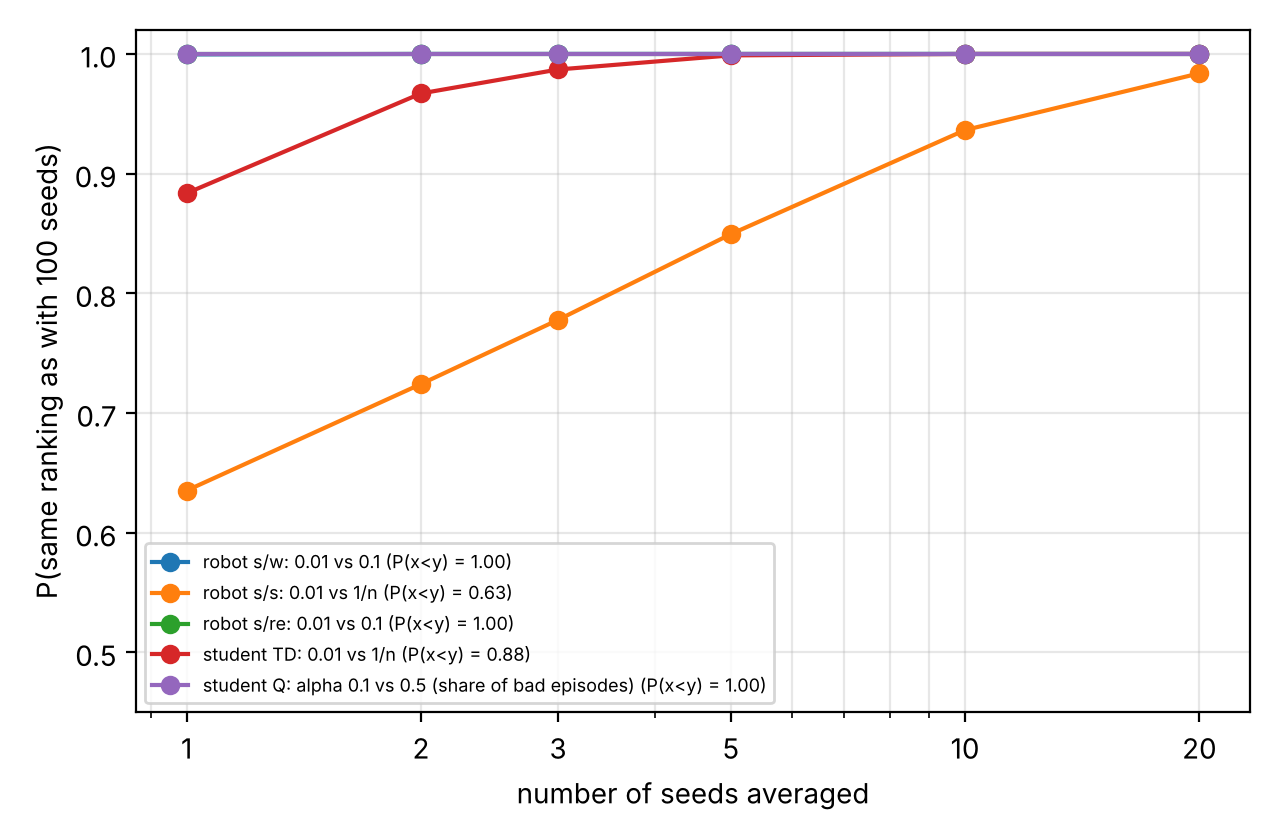
\includegraphics[width=0.66\textwidth]{seeds_agreement.png}
\caption{Probability that the mean over $k$ random seeds ranks two settings like the mean over 100 seeds (bootstrap, 5\,000 resamples). The three comparisons with $P(x<y) = 1$ are all at 1 and their lines are on top of each other.}
\label{fig:agreement}
\end{figure}

For three of the five comparisons of Figure~\ref{fig:agreement} one seed is enough: the probability of improvement is 1, every single seed ranks them in the same way. For the student, $\alpha = 0.01$ against $1/n$ has $P(X < Y) = 0.88$, and the ranking with one seed agrees with the 100-seed ranking 88\% of the time, 97\% with two seeds and 99\% with three. The hard one is s/s on the robot, $\eta = 0.01$ against $1/n$, with $P(X < Y) = 0.63$: one seed agrees 64\% of the time, five seeds 85\%, ten seeds 94\% and twenty seeds 98\%.

Note that with one seed the agreement is just the probability of improvement (0.64 against 0.63, 0.88 against 0.88), which is obvious once you see it. A rough rule from our five cases: if $P(X<Y)$ is above $0.85$, three seeds are enough; around $0.6$ you need something like twenty. The problem is that you only know $P(X<Y)$ after running many seeds.

\subsection{Means and standard deviations can hide a lot}

\begin{figure}[htbp]
\centering
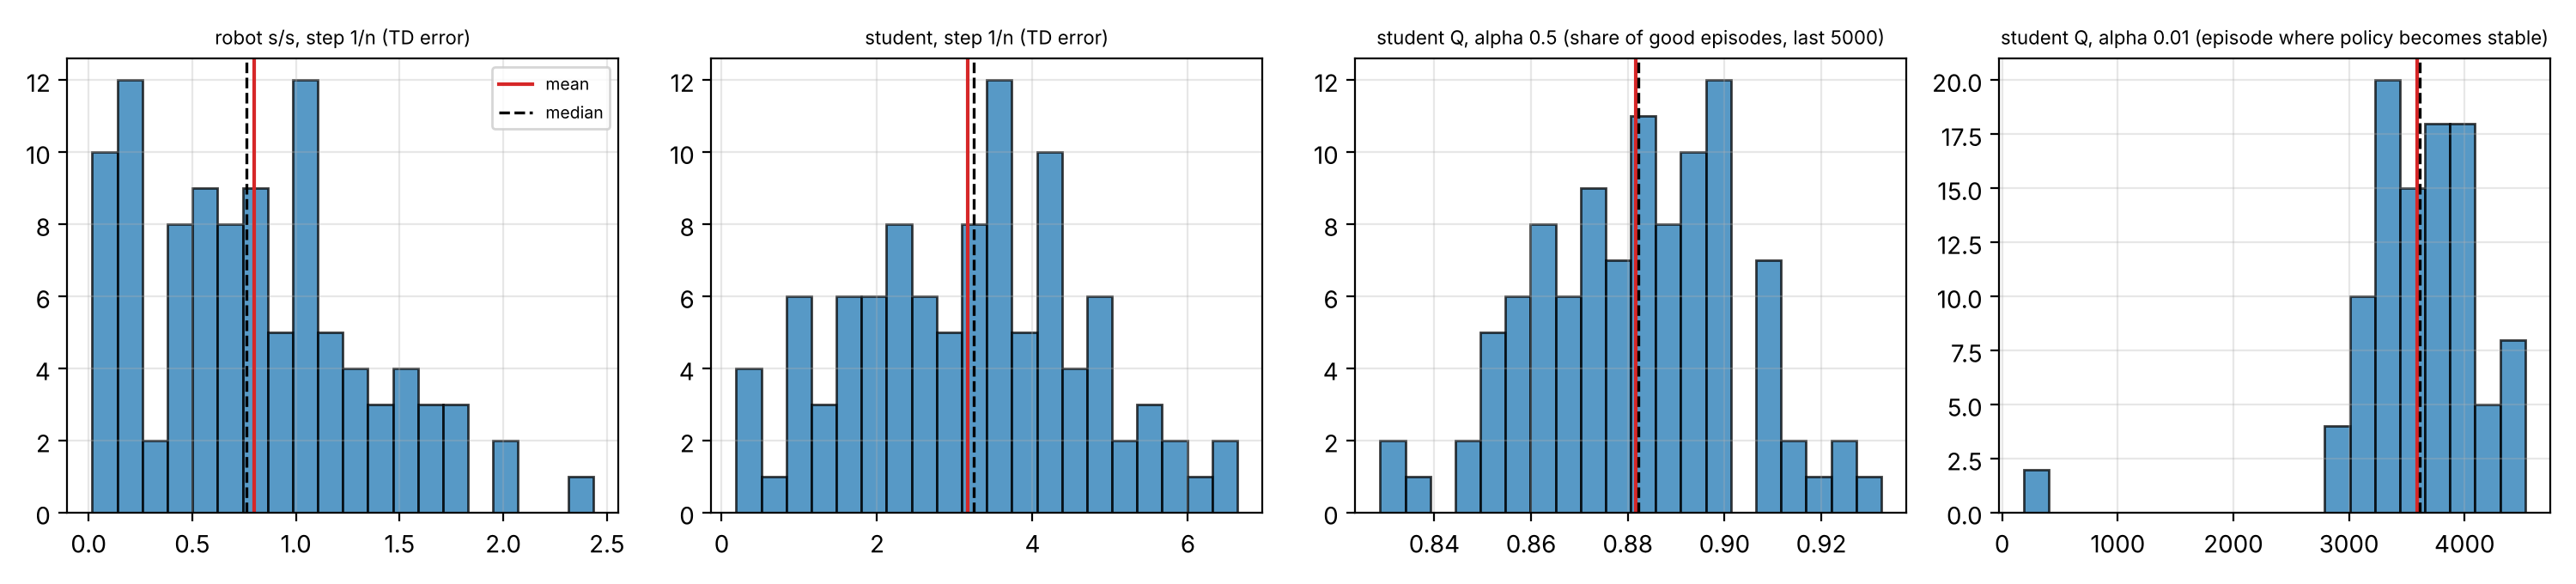
\includegraphics[width=\textwidth]{seeds_shapes.png}
\caption{Distribution over 100 seeds of four quantities of the report. Red: mean, dashed: median.}
\label{fig:shapes}
\end{figure}

Figure~\ref{fig:shapes} shows four distributions over the 100 seeds. The TD error of $1/n$ on s/s goes from $0.02$ to $2.44$, with mean $0.80$ and standard deviation $0.53$. Written as $0.80 \pm 0.53$ it looks like a noisy but unimodal quantity, but in fact 23\% of the seeds are under $0.3$ and 35\% are above 1. The same step on the student is wide but symmetric ($3.17 \pm 1.49$, from $0.19$ to $6.64$), so there one seed can give anything between a very good and a very bad result. The episode where Q-learning with $\alpha = 0.01$ becomes stable is the opposite case: 98 seeds between 2\,854 and 4\,524 and two seeds at 190 and 249, where the exploration found the reward of state 6 early. Those two seeds pull the standard deviation up to 625, while the interquartile mean (3\,628) and the median (3\,615) are hardly affected. None of this is surprising for people who work on RL evaluation \cite{agarwal2021}, but we would not have guessed it on problems this small.
